




\section{Motivation}
%%%%%%%%%%%%%%%%%%%%%%%%%%%%%%%%%%%%%%%%%%%%%%%%%%%%%%%%%%%%%%%%%%%%%%
\begin{frame}[label=intro30]{The first and third person routes to KT}

KT is a theory of \textit{structured experience} stemming from Algorithmic Information Theory (AIT). \vspace{0.5cm}

\begin{minipage}{0.5\linewidth}
    Two logical routes concern us:
    \vspace{0.5cm}
    
    \textbf{The first route} is the subjective, first-person route (1P, \textit{experience}).
    \vspace{0.5cm}
    
    \textbf{The second route} is the objective, third-person perspective (3P, \textit{life}).
\end{minipage}%
\hfill
\begin{minipage}{0.45\linewidth}
    \centering
    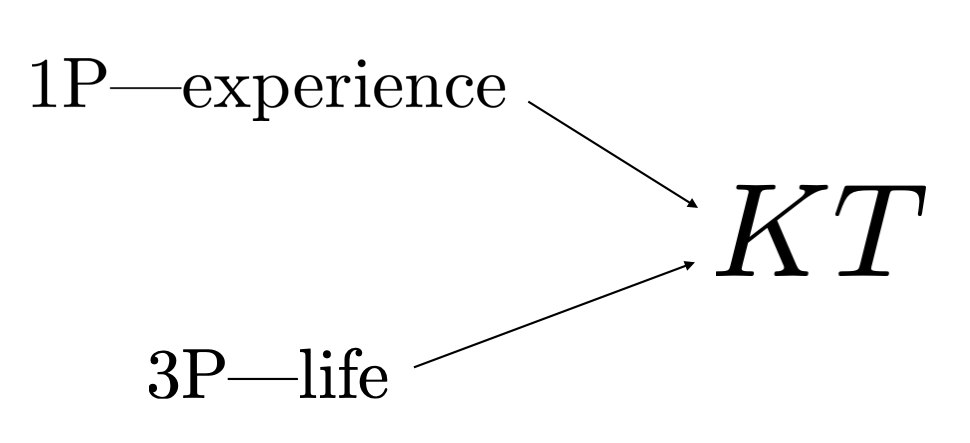
\includegraphics[height=3.2cm]{img/KT.png}
\end{minipage}

\end{frame}
%%%%%%%%%%%%%%%%%%%%%%%%%%%%%%%%%%%%%%%%%%%%%%%%%%%%%%%%%%%%%%%%%%%%%%
\begin{frame}[label=intro]{The subjective route to KT: first person experience}
	We start from the \textbf{fact of experience}---the first person (1P), subjective standpoint \citep{Ruffini2017}.  \vfill
	
	From the self-evidence of our own experience, the ``what it's like to be'', we assume that there is a primordial (pure, unstructured) form of experience.\vfill
	
    \begin{alertblock}{Warning:  \textbf{We assume {\em there exists experience.}} } 
	KT does not address the hard problem of consciousness.  
	\end{alertblock}
	

\end{frame}

%%%%%%%%%%%%%%%%%%%%%%%%%%%%%%%%%%%%%%%%%%%%%%%%%%%%%%%%%%%%%%%%%%%%%%
\begin{frame}[label=intro2]{Structured experience (\SEP)}
 We aim to build a theory around the notion of 
{\em structured experience}---where {\em mathematics} and experience meet.  \vfill

{\bf Mathematics:}  The science of structure, order, and relation  \cite{davisMathematicalExperience1981}.  \vfill

%Following the phenomenological tradition, w
We observe that all we have access to is \textit{information} and that experience is {\em structured}. \vfill

	\begin{definition}[\textbf{Structured experience }(\SEP)]
The phenomenal structure of consciousness  encompassing the spatial, temporal, and conceptual organization of our experience  \citep{VanGulick:2016aa}. 
	\end{definition}

	

\end{frame}


% \begin{frame}{Structured experience (\SEP)}
% { \begin{center}
%          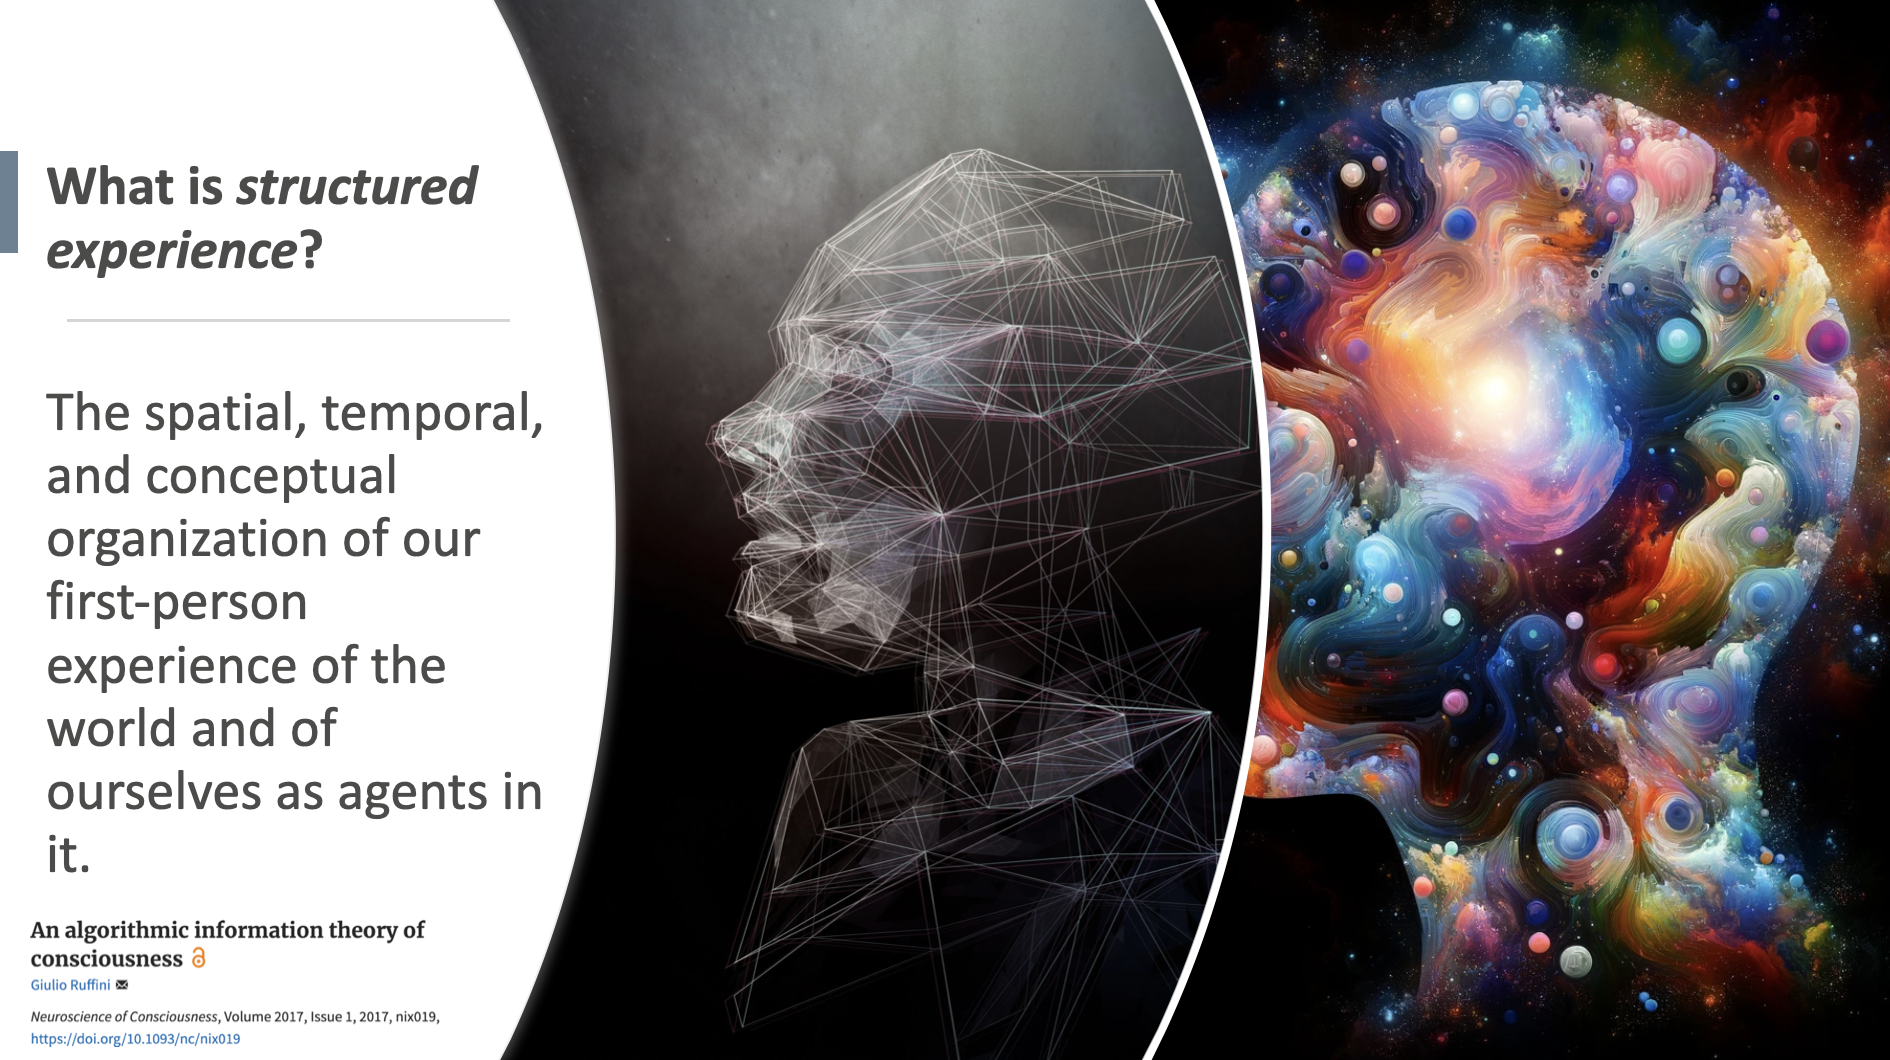
\includegraphics[height=6.5cm]{img/Structured_exp_def.png}
%      \end{center}}
    
% \end{frame}
%%%%%%%%%%%%%%%%%%%%%%%%%%%%%%%%%%%%%%%%%%%%%%%%%%%%%%%%%%%%%%%%%%%%%%
% \begin{frame}[label=intro3]{Scientific strategy for the study of \SEP}
% This definition of \SEP can be empirically explored in reporting humans, and  we   aim to characterize it with methods  applicable to a broad range of systems.  \vfill

%   The strategy will be to quantify the structure of experience from {\bf 1P reports}  in humans and attempt to associate it with 3P data (e.g., EEG, fMRI, or behavior) using mechanistic insights derived from neuroscience and mathematics --- \textbf{Computational neurophenomenology}.  \vfill
  
%   We can then study (3P) other systems (non-reporting humans, other living species or artificial agents) %. \vfill
%   %
%   %With  bases for comparison  of the state and behavior of an artificial agent and that of an \SEP-reporting human, we
%   for an educated guess about the agent's \SEP.

% \end{frame}

%%%%%%%%%%%%%%%%%%%%%%%%%%%%%%%%%%%%%%%%%%%%%%%%%%%%%%%%%%%%%%%%%%%%%%
\begin{frame}[label=intro4]{The objective route to KT (3P): persistence and life}
Alternatively, we can start by attempting to define what {\em life} is.\vfill

\textbf{What remains after the passage of computational eons} must rightfully be called a {\em persistent pattern}.\vfill

There may be several types of such patterns. Some seem rather impervious to the world, such as protons or diamonds. Others are rather interactive. \vfill

\begin{figure}
    \centering
    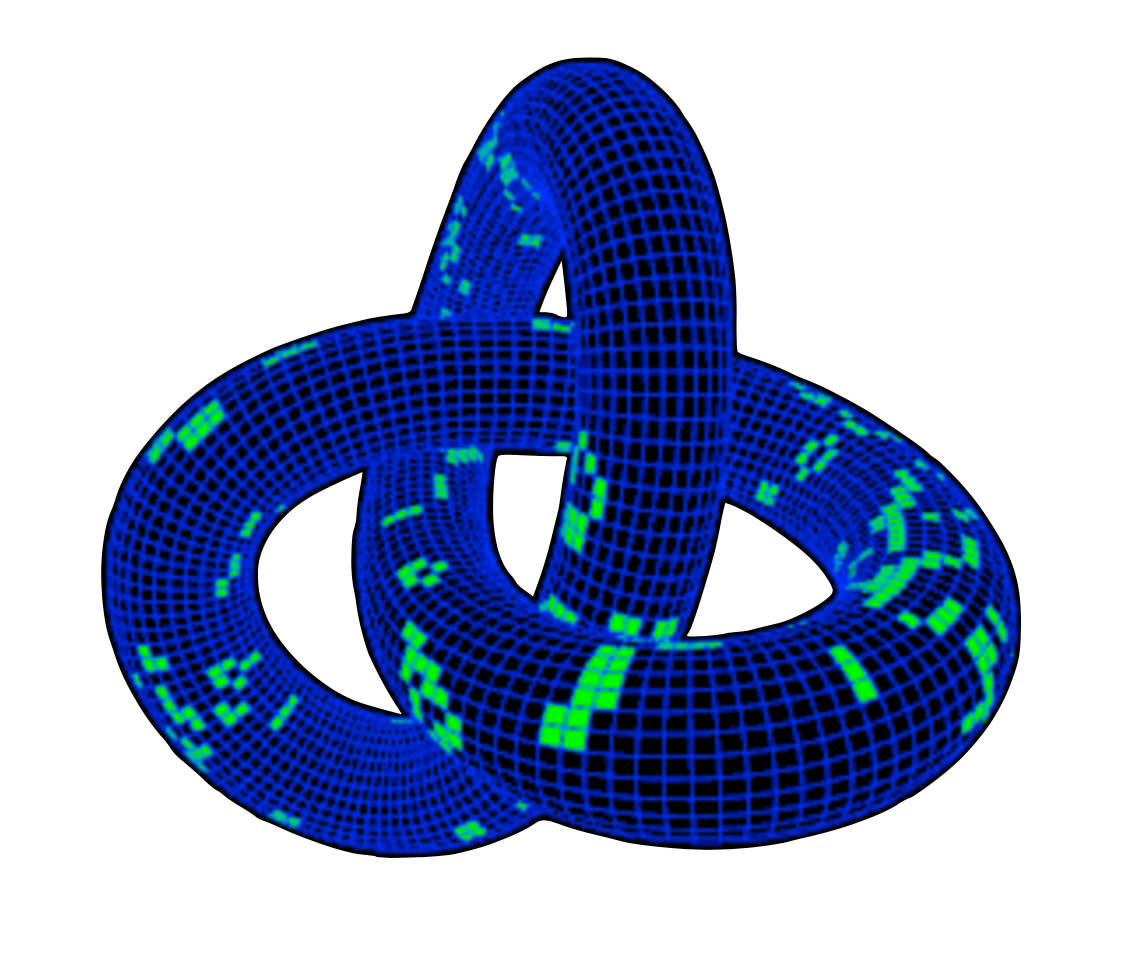
\includegraphics[width=0.25\linewidth]{toruslife.png}
\end{figure}
\end{frame}

\begin{frame}[label=intro4]{The objective route to KT (3P): persistence and life}
\begin{definition}[\textbf{Life}]
Life refers to algorithmic patterns that readily interact but persist by capturing structure in the World they inhabit to \textit{stay} (homeo- and tele-homeostasis).  \end{definition}\vfill

 {\bf The connection with the first viewpoint is that, in KT, this {generalized definition of \em life is what is capable of \SEP}}. \vfill 
 
 As part of our program, we should study the algorithmic emergence of life. 
\end{frame}

%%%%%%%%%%%%%%%%%%%%%%%%%%%%%%%%%%%%%


